\documentclass[15pt]{extarticle}
\usepackage{graphicx}
\usepackage[utf8]{inputenc}
\usepackage[T1]{fontenc}
\usepackage{natbib}
\usepackage{lmodern}
\usepackage{titlesec}
\usepackage{tabularx}

\titlespacing*{\section}
{0pt}{10.0ex plus 1ex minus .2ex}{2.0ex plus .1ex minus .1ex}
\titlespacing*{\subsection}
{0pt}{6.0ex plus 1ex minus .2ex}{1.0ex plus .1ex minus .1ex}

% For enumerations with section number.
%\usepackage{enumitem}
%\setenumerate[1]{label=\thesection.\arabic*.}
%\setenumerate[2]{label*=\arabic*.}


\renewcommand{\familydefault}{\sfdefault}

\usepackage{geometry}
 \geometry{
 a4paper,
 left=20mm,
 right=20mm,
 top=20mm,
 bottom=30mm,
 }

\usepackage[colorlinks = true,
            linkcolor = blue,
            urlcolor  = blue,
            citecolor = black,
            anchorcolor = blue]{hyperref}

\setlength{\parskip}{0.5em}
\renewcommand{\baselinestretch}{1.2}

\title{DMBSim v1.0 tutorial 1}
\author{Enrico Mattea}
\date{October 2021}


\begin{document}

%\maketitle

\begin{titlepage}
    
\includegraphics[width=5cm]{unifr_logo}
    \par
    \vspace{2.0cm}
	\centering
	{\huge\textbf{DMBSim v1.0\\}}
	\vspace{0.3 cm}
	{\large \textbf{Tutorial 1:} installation and simulation of single-year glacier mass balance\\}
	\vspace{2.4 cm}
	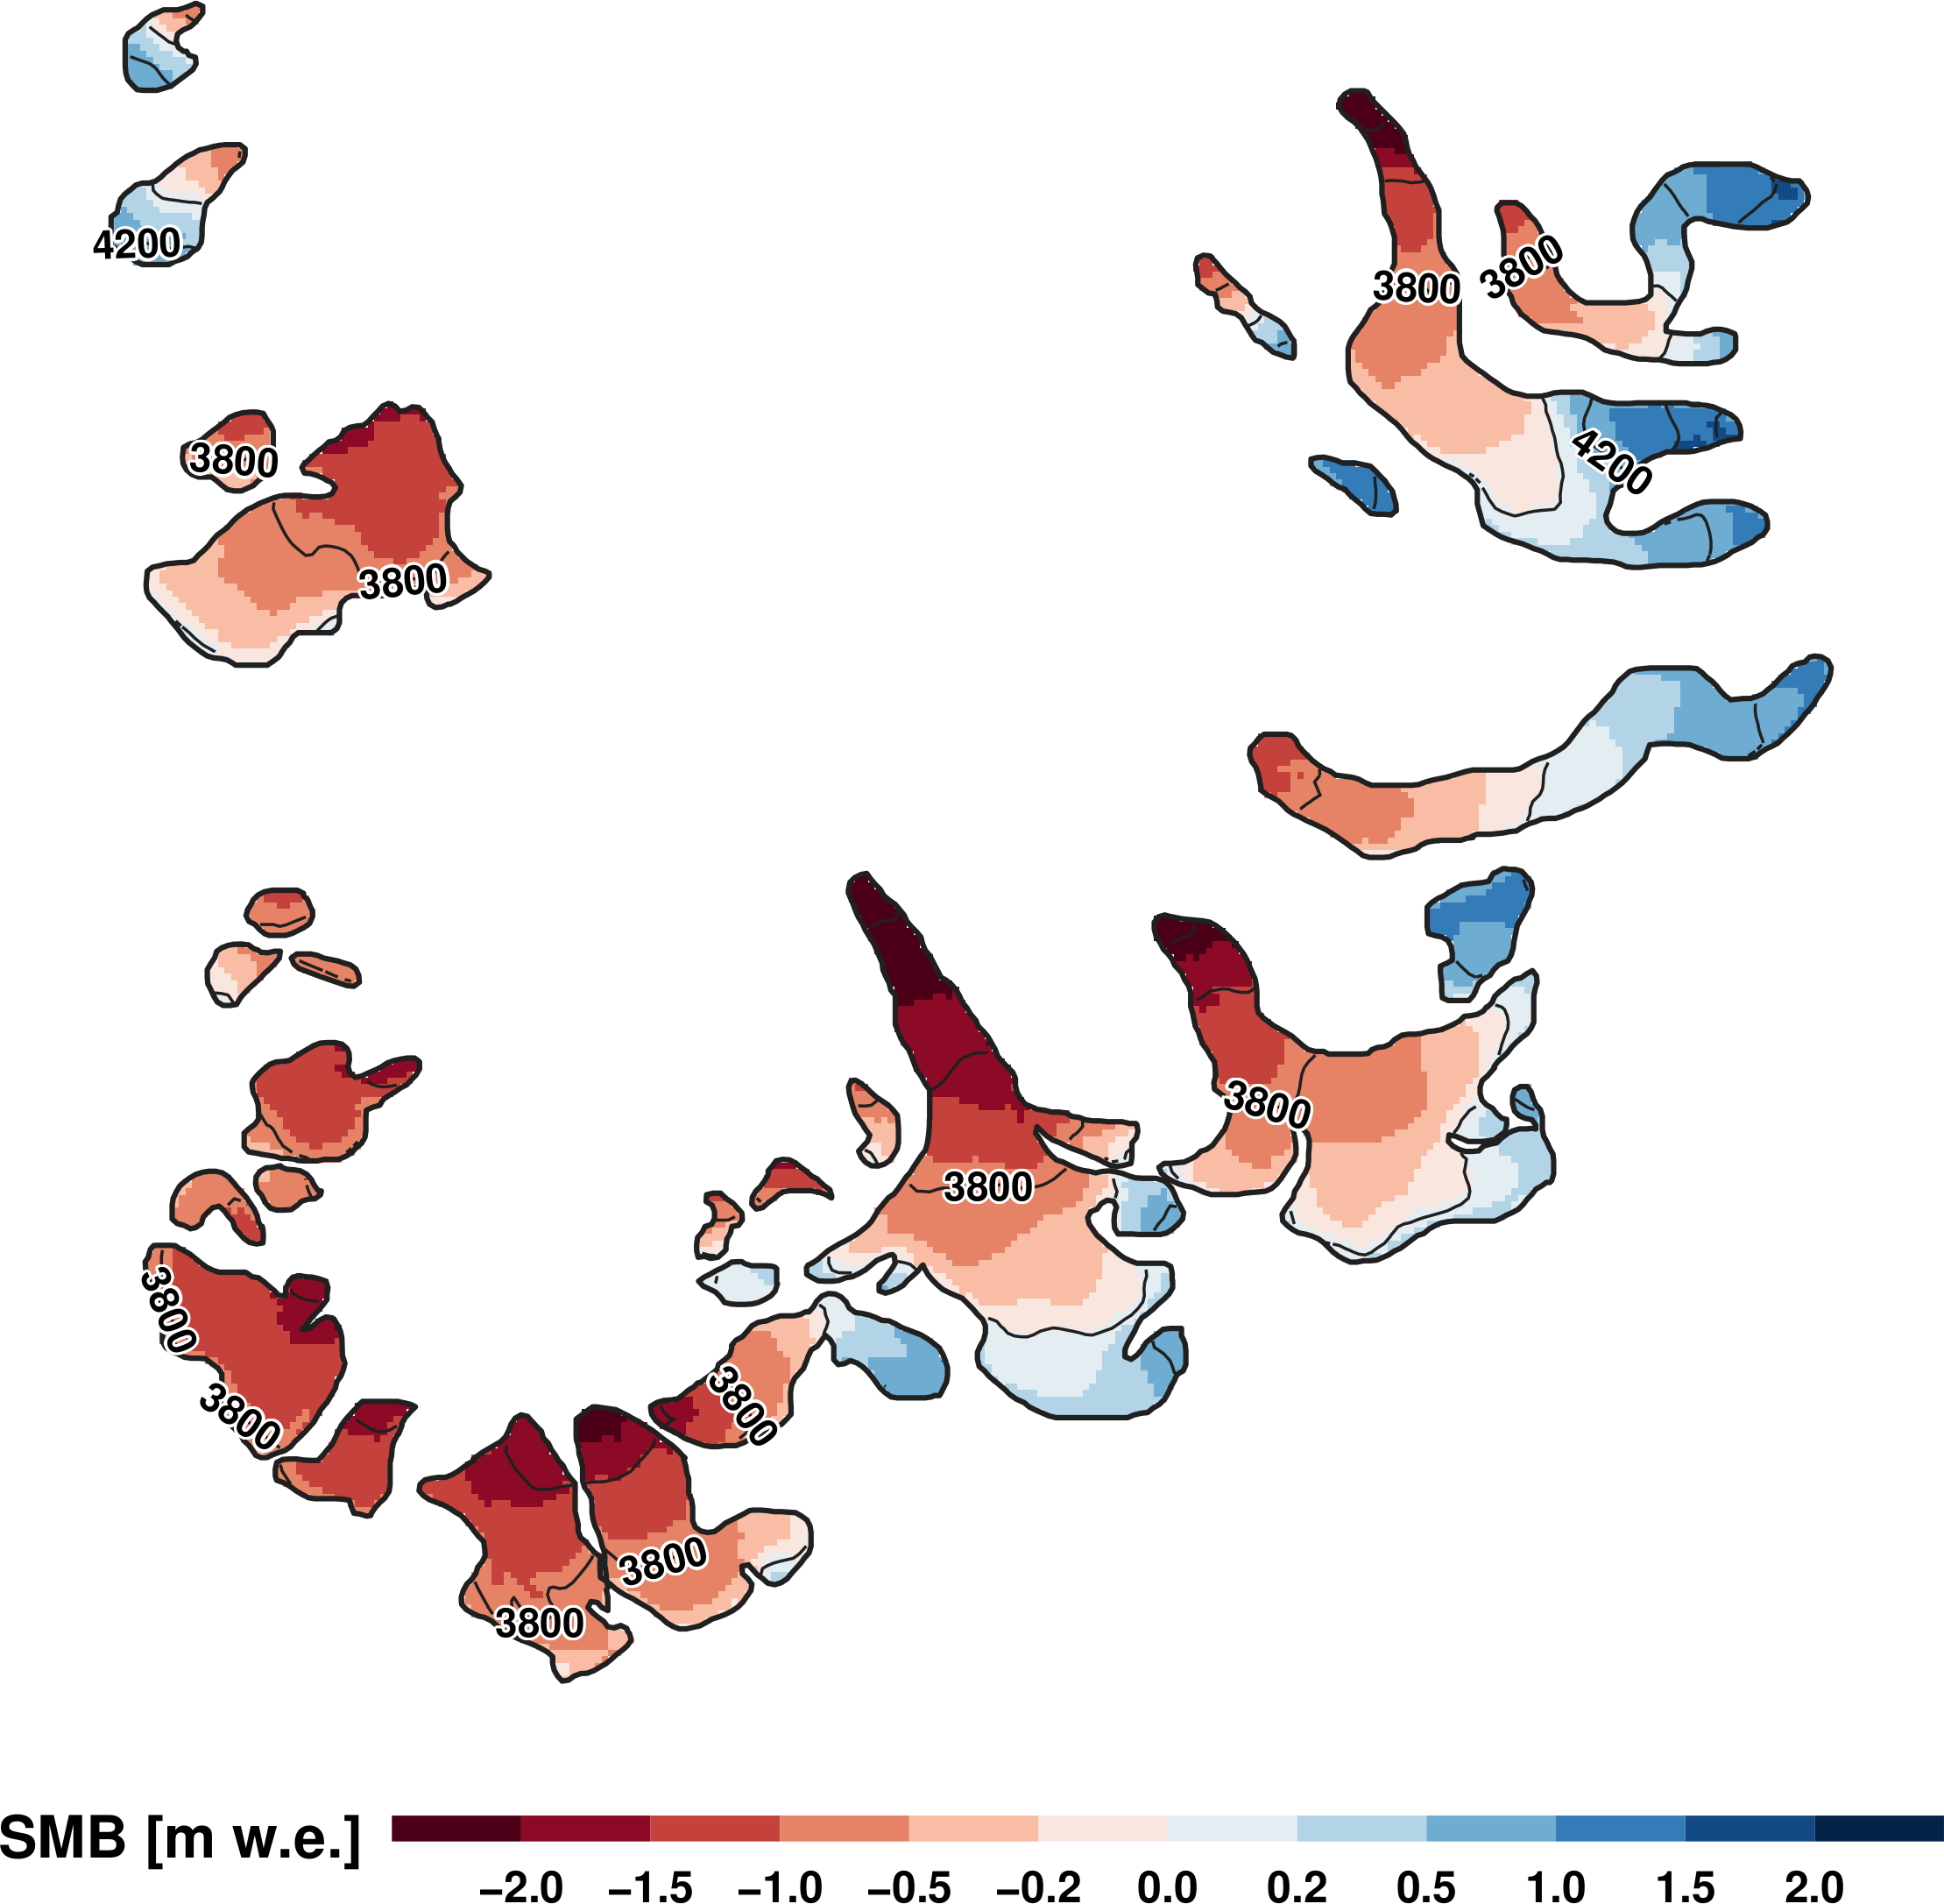
\includegraphics[width=12cm]{f0_cover_image}\par
	\vspace{2.1 cm}
	{\normalsize \textbf{Enrico Mattea}\\}
	{\normalsize \textit{enrico.mattea@unifr.ch\\}}
	\vspace{0.6 cm}
	{\normalsize October 2021}


	\vfill

\end{titlepage}


\section{Introduction}
In this first tutorial we are going to install the model and then simulate the mass balance of Yakarcha glacier (Pamir-Alay) over one year (2020).
We will proceed like this:
\begin{itemize}
    \item Install the \textbf{required programs}
    \item Prepare the model \textbf{input files}
    \item Setup the model \textbf{parameters}
    \item \textbf{Run the model.}
\end{itemize}

\clearpage
\section{Installation}
We install the required programs in this order: first \textbf{R}, then \textbf{RStudio}, finally the \textbf{R packages} which are used by the model. If you have already installed some of the programs, you can skip the corresponding sections.
To install everything, you need an internet connection and at least 2 GB of free disk space. \textbf{All steps below are required}, if any one of them goes wrong you should correct it or the model will not work properly.

\begin{itemize}
    \item \textbf{Download and install R.} For the Windows operating system, download the installer from \href{https://cran.rstudio.com/bin/windows/base/}{this page.} For other operating systems, see \href{https://cran.rstudio.com/}{the landing page.} After download, open the installer and follow the instructions until installation is complete.
    \item \textbf{Download and install RStudio.} Go to \href{https://www.rstudio.com/products/rstudio/download/#download}{this page} and download the installer which corresponds to your operating system (usually Windows 10). Again, open the installer and proceed until RStudio is installed.
    \item To install the \textbf{required R packages} we use the program \textit{install\_packages.R}, which you can find inside \textit{utils\textbackslash} in the model folder. Open file \textit{install\_packages.R} in RStudio and click on the \textit{Source} button (Fig. \ref{fig:f1_rstudio_source}) to run the program.
    
\begin{figure}[h]
    \centering
    \includegraphics[width=0.8\textwidth]{f1_rstudio_source}
    \caption{The Source button in RStudio.}
    \label{fig:f1_rstudio_source}
\end{figure}
    
    \item The program will download and install several packages \textbf{automatically}. After some time it will open a new window to install "Rtools": simply click "Next" and "Install" to proceed.
    \item When \textit{install\_packages.R} has finished (message \textbf{"All packages installed succesfully!"}), you should \textbf{close RStudio.}
\end{itemize}


\clearpage
\section{Input files}
\subsection{Overview}
For the mass balance model we have to provide some input data. It is \textbf{important to put the input data in the right place:} all the input data should go \textbf{inside the model folder,} in a folder called \textit{input\textbackslash}. There \textbf{we create a sub-folder with the name of the glacier:} \textit{input\textbackslash yakarcha\textbackslash}. The name of the glacier should \textbf{not have any white spaces} (so for example we would use \textit{batysh\_sook} instead of \textit{batysh sook}). Now we prepare the following input data for the model:
\begin{itemize}
    \item a text file with the daily \textbf{meteorological series}
    \item a text file with the \textbf{mass balance measurements}
    \item a \textbf{glacier outline} in vector format (shapefile)
    \item an \textbf{elevation grid} (called "DHM": the full rectangle covering the glacier region, with no missing values)
    \item a grid of \textbf{surface type} (ice, firn, debris)
    \item 365 grids of \textbf{daily solar radiation.}
\end{itemize}
\textbf{The first two} (meteo and mass balance) are provided together with this tutorial, in folder \textit{tutorial1\_input\textbackslash yakarcha\textbackslash}. To prepare \textbf{the last four} (outline, elevation, surface type and radiation grids) we will use the program \textit{make\_input.R}, located in the model folder \textit{utils\textbackslash}. This program will create and process the files \textbf{automatically.}

\subsection{Meteorological series}
\label{sect:input_meteo}
The meteorological series goes into a simple text file, with 5 columns: \textbf{year, day of year (1-365), hour, temperature, precipitation} (Fig. \ref{fig:f2_meteo_file}). We call this meteo file \textit{weather\_yakarcha.dat} and we place it into a new folder: \textit{input\textbackslash yakarcha\textbackslash weather\textbackslash}. The model works at \textbf{daily resolution}: "temperature" is the daily mean temperature, "precipitation" the total daily precipitation (in mm w.e., including solid and liquid), and the "hour" column has a constant value 12 for every day. As you can see in Fig. \ref{fig:f2_meteo_file}, \textbf{the meteo file can have a comment text} at the beginning, to explain what is inside. Later we can tell the model to ignore these comment lines.

\textbf{Note:} the meteo file must have \textbf{data for every day} which is modeled, or the model will refuse it. The model always includes \textbf{the entire hydrological year} (1 October-30 September) in the simulation. The model also includes \textbf{the entire period measured} at the stakes. We want to model year 2020, with mass balance stakes visited on 14.8.2019 and again on 13.9.2020. Then we need at least meteo data for every day from 14.8.2019 to 30.9.2020. This is the meteo data which \textbf{must be present}, but in the meteo file there can also be (in addition) \textbf{the data of other days/years:} the model will select the correct data automatically.

\begin{figure}[h]
    \centering
    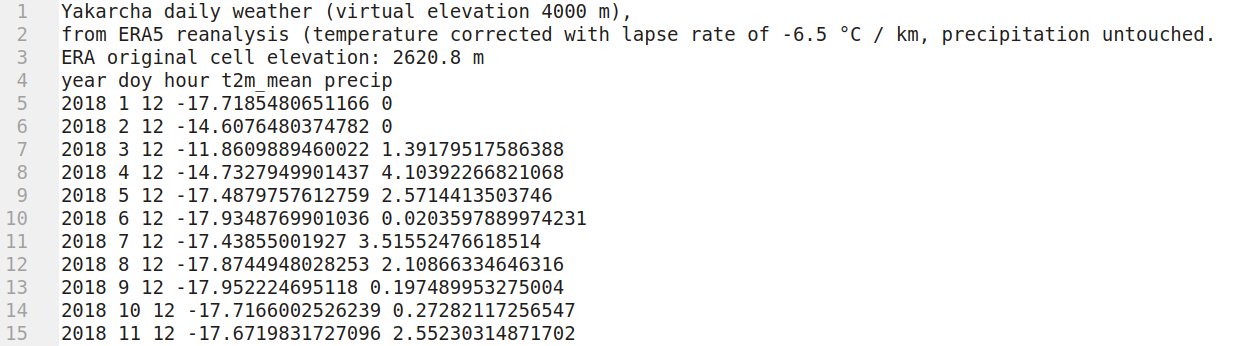
\includegraphics[width=1.0\textwidth]{f2_meteo_file}
    \caption{The first lines of the meteo file.}
    \label{fig:f2_meteo_file}
\end{figure}


\subsection{Mass balance measurements}
\label{sect:input_mb}
The mass balance measurements go into a simple text file, with 8 columns: \textbf{point name} (with no spaces), \textbf{start date, end date, X coordinate, Y coordinate, altitude, measured change at the stake, measured density} (Fig. \ref{fig:f3_massbal_file}). We call this file \textit{mb\_yakarcha.dat} and we place it into a new folder: \textit{input\textbackslash yakarcha\textbackslash massbalance\textbackslash}. We are modeling the year 2020, so the "start date" is in summer 2019, the "end date" in summer 2020. The format is "day.month.year", such as 14.8.2019 for 14 August 2019. \textbf{Note} that in (Fig. \ref{fig:f3_massbal_file}) some measurements (J8, J9 and J10) have a \textbf{special start date NA}: this is used for the summer snow pits and snow probes, where the "starting date" is usually not known (the measured change in this case is defined from the surface \textbf{at the end of the previous melting season}). Thus, for all measurements with start date NA \textbf{the model automatically sets the start date} at the end of the previous melting season.

The \textbf{X and Y coordinates} should be \textbf{in meters} (UTM: for Yakarcha, we use UTM zone 42N, which is also called EPSG:32642). The \textbf{measured change at the stake} is \textbf{in centimeters}, $>$ 0 for accumulation and $<$ 0 for ablation. \textbf{Density} is in g cm\textsuperscript{-3} (water = 1, ice = 0.9). Our measurements at Yakarcha are already in centimeters water-equivalent (cm w.e.), so we use density = 1.

\begin{figure}[h]
    \centering
    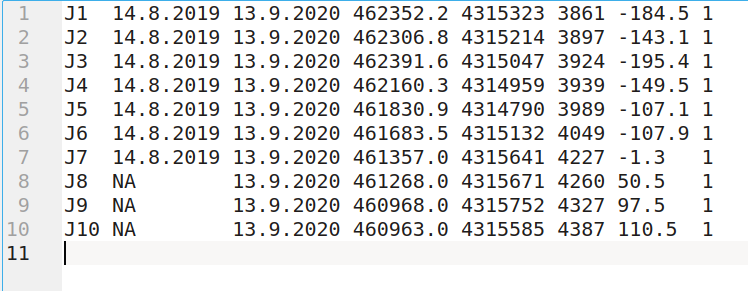
\includegraphics[width=0.55\textwidth]{f3_massbal_file}
    \caption{The file with the mass balance measurements.}
    \label{fig:f3_massbal_file}
\end{figure}



\subsection{Glacier outline}
\label{sect:input_outline}
The glacier outline is a polygon which delimits the glacier surface (Fig. \ref{fig:f6_qgis_polygon}). To create the outline shapefile we \textbf{draw it manually} over a satellite image of the glacier, taken by Sentinel-2. We download the image from the EarthExplorer portal. To draw the outline we use the program \href{https://qgis.org}{QGIS}, but you can also use ArcGIS or any other program you like. \textbf{Note:} if you already have a method to create the glacier outline shapefile, you can use it instead of the steps below.

\begin{itemize}
    \item If you don't have an account on EarthExplorer, first create one here: \href{https://ers.cr.usgs.gov/register}{https://ers.cr.usgs.gov/register}.
    \item Login here: \href{https://ers.cr.usgs.gov/login}{https://ers.cr.usgs.gov/login}.
    \item Now go to the portal: \href{https://earthexplorer.usgs.gov/}{https://earthexplorer.usgs.gov/}.
    \item On the map, we move to the glacier (38° 59' North, 68° 34' East).
    \item We click three points to draw a triangle over the glacier (Fig. \ref{fig:f4_earthexplorer_points}).
    
    \begin{figure}[h!]
    \centering
    \includegraphics[width=0.8\textwidth]{f4_earthexplorer_points}
    \caption{The EarthExplorer portal at Yakarcha glacier.}
    \label{fig:f4_earthexplorer_points}
    \end{figure}
    
    \item In the left column, we select \textbf{Data Sets $\rightarrow$ Sentinel $\rightarrow$ Sentinel-2}, then we click \textbf{Results} (Fig. \ref{fig:f5_earthexplorer_datasets}).
    \item In the left column a list of images appears, on many pages. We choose the one called\\ \textit{L1C\_T42SVJ\_A027301\_20200913T060752}, with "Acquisition Date" 2020/09/13, and we download the "L1C Tile in JPEG2000 format".
    \item We extract the zip file and we open in QGIS the file located under GRANULE \textit{$\rightarrow$ \\ L1C\_T42SVJ\_A027301\_20200913T060752 $\rightarrow$ IMG\_DATA $\rightarrow$ T42SVJ\_20200913T060641\_B04.jp2}.
    \item In QGIS we move to the glacier and we click on \textbf{Layer $\rightarrow$ Create Layer $\rightarrow$ New Shapefile Layer}, geometry type \textbf{Polygon}, file name \textit{outline\_yakarcha\_2020.shp}, coordinates system \textbf{EPSG:32642}.
    \item Then we manually trace the glacier outline: we click on \textbf{Toggle Editing} and \textbf{Add Polygon Feature}, then we draw the polygon following the glacier outline (Fig. \ref{fig:f6_qgis_polygon}).
    \item Finally we click again on \textbf{Toggle Editing} and we save the changes.
\end{itemize}
The shapefile is made of 5 separate files, which end with .shp, .shx, .dbf, .prj and .cpg. We keep them ready since we will use them in the next steps.

\begin{figure}[hp]
    \centering
    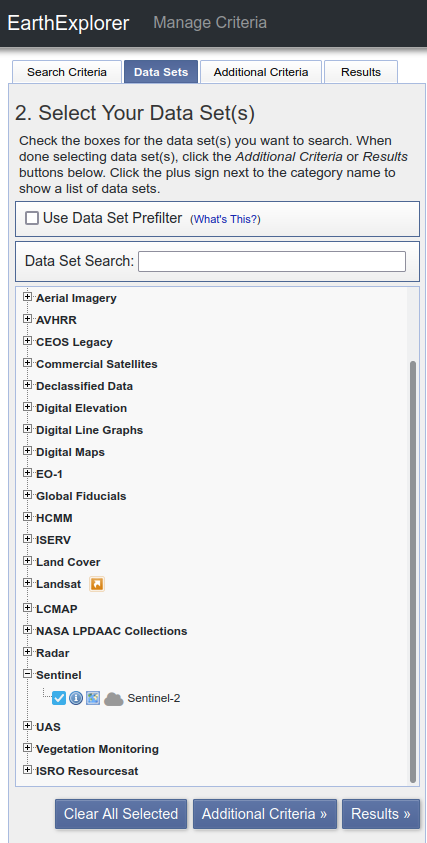
\includegraphics[width=0.3\textwidth]{f5_earthexplorer_datasets}
    \caption{The EarthExplorer portal: selecting the Sentinel-2 dataset.}
    \label{fig:f5_earthexplorer_datasets}
\end{figure}

\begin{figure}[hp]
    \centering
    \includegraphics[width=0.85\textwidth]{f6_qgis_polygon}
    \caption{The glacier outline traced in QGIS over the Sentinel-2 image. The red circle shows the \textbf{Toggle Editing} and \textbf{Add Polygon Feature} buttons.}
    \label{fig:f6_qgis_polygon}
\end{figure}


\subsection{DEM}
\label{sect:input_dem}
The glacier topography is defined by a DEM file. We download this file from EarthExplorer: the procedure is the same as for the Sentinel-2 image (see above), but the file is located under \textbf{Data Sets $\rightarrow$ NASA LPDAAC collections $\rightarrow$ ASTER collections $\rightarrow$ Aster Global DEM V3} (don't forget to \textbf{remove} the previous Data Sets \textbf{(Sentinel $\rightarrow$ Sentinel-2)} before clicking on \textbf{Results}). When you try to download the DEM, EarthExplorer can ask you to do a login: in this case you can register \href{https://urs.earthdata.nasa.gov/users/new}{here}. We download the GeoTIFF format and extract the .zip archive. The important file is \textit{ASTGTMV003\_N38E068\_dem.tif}, for the moment we leave it where it is: we will use it in the next step.

\textbf{Note:} if you want to use a different DEM, you can have a look at \href{https://www.usna.edu/Users/oceano/pguth/md_help/html/global_dems.html}{this excellent list}. A very useful download service for global DEMs is provided by the \href{https://portal.opentopography.org/dataCatalog?group=global}{OpenTopography} website. It is important to use a DEM with \textbf{no gaps/voids/NAs}, these will not work in the mass balance model.

\subsection{Program \textit{make\_input.R}}
\label{sect:input_make_input}
We use program \textit{make\_input.R} to prepare the input files which are still missing.\\\textbf{Note:} it is \textbf{not needed to change the coordinate system} of any file: \textit{make\_input.R} will always \textbf{adjust} all coordinate systems \textbf{automatically}.
\begin{itemize}
    \item First we open with RStudio the file \textit{make\_input.R} (inside folder \textit{utils\textbackslash}).
    \item We click on \textbf{Run App} (Fig. \ref{fig:f7_rstudio_runapp}).
    \item A new window opens: \textbf{Mass balance model assistant}.
    \item We enter the \textbf{glacier name}. This is the same as the folder where we are putting the input files: \textit{yakarcha}.
    \item We enter the \textbf{modeled year}: 2020.
    \item We click button \textbf{Choose one or more input DEM files} and we select the file which we have just downloaded: \\\textit{ASTGTMV003\_N38E068\_dem.tif}. The program can also use \textbf{multiple input DEM files} in case the glacier is divided across several tiles: if you provide more than one input DEM, they are merged together before processing.
    \item We click button \textbf{Choose input glacier shapefile} and we select the outline shapefile which we have created before: \textit{outline\_yakarcha\_2020.shp}.
    \item We don't touch the other buttons, in the text field we \textbf{choose a margin size} of 100 m around the outline.
    \item We leave empty the \textbf{grid cell size}, it is computed automatically. We can also force a specific cell size by writing a value (in meters).
    \item We select \textbf{Compute daily potential solar radiation}.
    \item Finally we click on button \textbf{RUN!} (Fig. \ref{fig:f8_make_input}).
    \item The program is now working, it can take a few minutes. You can \textbf{follow the progress in the big window of RStudio}.
    \item When the program has finished (notification \textbf{Processing finished}), inside the \textit{utils\textbackslash} folder there is a new folder, called \textit{yakarcha\textbackslash}. This contains folders \textit{dhm\textbackslash}, \textit{outline\textbackslash}, \textit{radiation\textbackslash} and \textit{surftype\textbackslash}. We \textbf{move} all these (the entire folder \textit{utils\textbackslash yakarcha\textbackslash}) to the folder \textit{input\nolinebreak\textbackslash\nolinebreak yakarcha\textbackslash.}
    \item In the end \textbf{the input folder looks like Fig. \ref{fig:f9_input_folder}:} under \textit{input\textbackslash yakarcha\textbackslash} there are 6 folders (\textit{dhm\textbackslash}, \textit{massbalance\textbackslash}, \textit{outline\textbackslash}, \textit{radiation\textbackslash}, \textit{surftype\textbackslash} and \textit{weather\textbackslash}). Folder \textit{outline\textbackslash} contains the shapefile, folder \textit{radiation\textbackslash} contains 365 radiation grids (the first one is called \textit{dir00124.tif}), and the other folders have only 1 file each.
\end{itemize}

\begin{figure}[h]
    \centering
    \includegraphics[width=0.85\textwidth]{f7_rstudio_runapp}
    \caption{The \textbf{Run App} button in RStudio.}
    \label{fig:f7_rstudio_runapp}
\end{figure}

\begin{figure}[h]
    \centering
    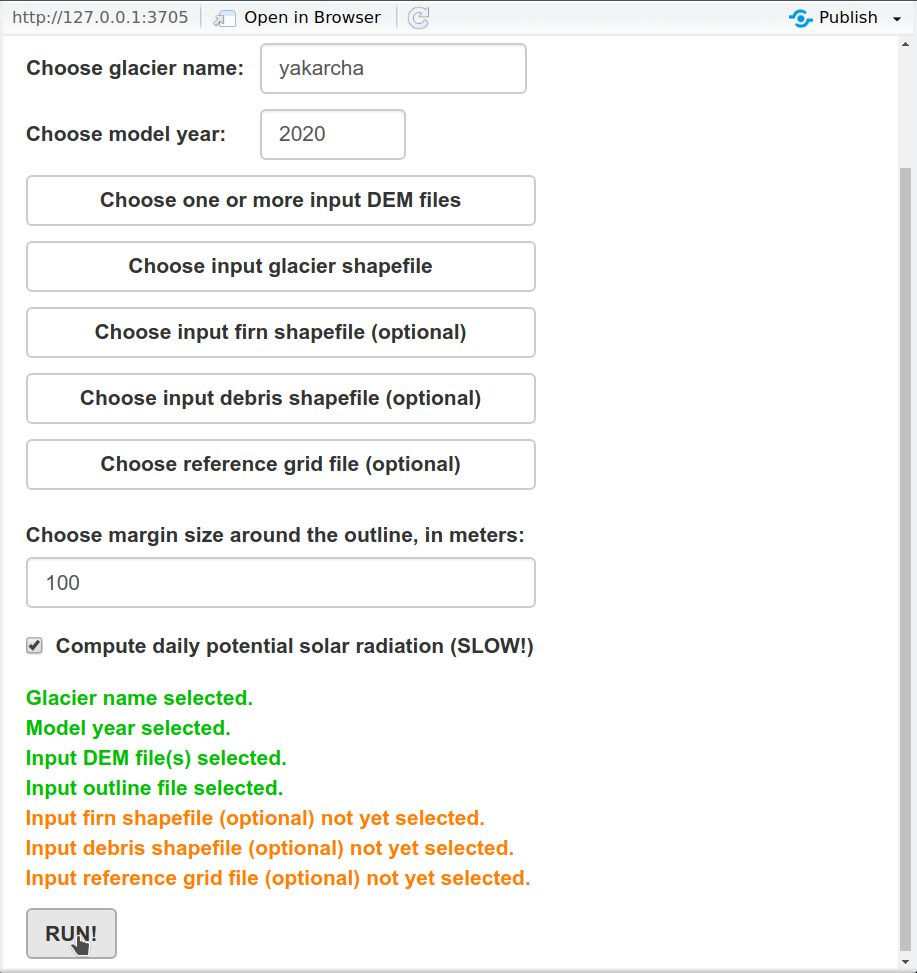
\includegraphics[width=0.55\textwidth]{f8_make_input}
    \caption{The \textit{make\_input.R} window after selecting the data, ready to click on \textbf{RUN!}}
    \label{fig:f8_make_input}
\end{figure}

\begin{figure}[h]
    \centering
    \includegraphics[width=0.7\textwidth]{f9_input_folder}
    \caption{The folder \textit{input\textbackslash yakarcha\textbackslash} after preparing all the input data.}
    \label{fig:f9_input_folder}
\end{figure}

\clearpage
\section{Model parameters}
The model parameters are set in a file called \textit{set\_params.R}, in the model folder. We \textbf{open this file in RStudio,} and we set the parameters as shown in Table \ref{table:t1_parameters}. There are many other parameters which can be set, but in this first simulation we only set the most important ones. When we change the parameters it is \textbf{important to keep the same format:} the \textbf{quotes} ("") and the \textbf{commas} (,) should \textbf{remain the same,} or the model will not work.

\begin{table}[h!]
\caption{model parameters which we change in this tutorial}
\label{table:t1_parameters}
\centering
\begin{tabularx}{\textwidth}{|l l X|} 
 \hline
 \textbf{Parameter name} & \textbf{Value} & \textbf{Explanation} \\ [0.5ex] 
 \hline
 name\_glacier & "yakarcha" & Glacier name, it is the \textbf{same as the folder} under \textit{input\textbackslash} \\ 
 \hline
 filename\_weather & "weather\_yakarcha.dat" & Name of the meteo file, which we set in section \ref{sect:input_meteo} \\
 \hline
 file\_weather\_nskip & 4 & Number of lines to skip in the meteo file, there are 4 lines which are not data (Fig. \ref{fig:f2_meteo_file}) \\
 \hline
 grids\_crs & 32642 & EPSG code of the coordinates system, 32642 is UTM zone 42N (Fig. \ref{fig:f10_epsg}). The full list of codes is \href{https://spatialreference.org/ref/epsg/?page=80}{here} \\
 \hline
 filename\_massbalance\_annual & "mb\_yakarcha.dat" & Name of the \textbf{file with the annual mass balance measurements,} which we set in section \ref{sect:input_mb}\\
 \hline
  filename\_massbalance\_winter & "" & Name of the file with the winter mass balance measurements. We don't have this so we leave it empty ("")\\
 \hline
  weather\_aws\_elevation & 4000 & Altitude of the meteo data. The Yakarcha file refers to an altitude of 4000 m\\
 \hline
  first\_year & 2020 & First year that we want to simulate: 2020\\
 \hline
  last\_year & 2020 & Last year that we want to simulate, we want to do just one year so it is again 2020\\
 \hline
\end{tabularx}
\end{table}

\begin{figure}[hp]
    \centering
    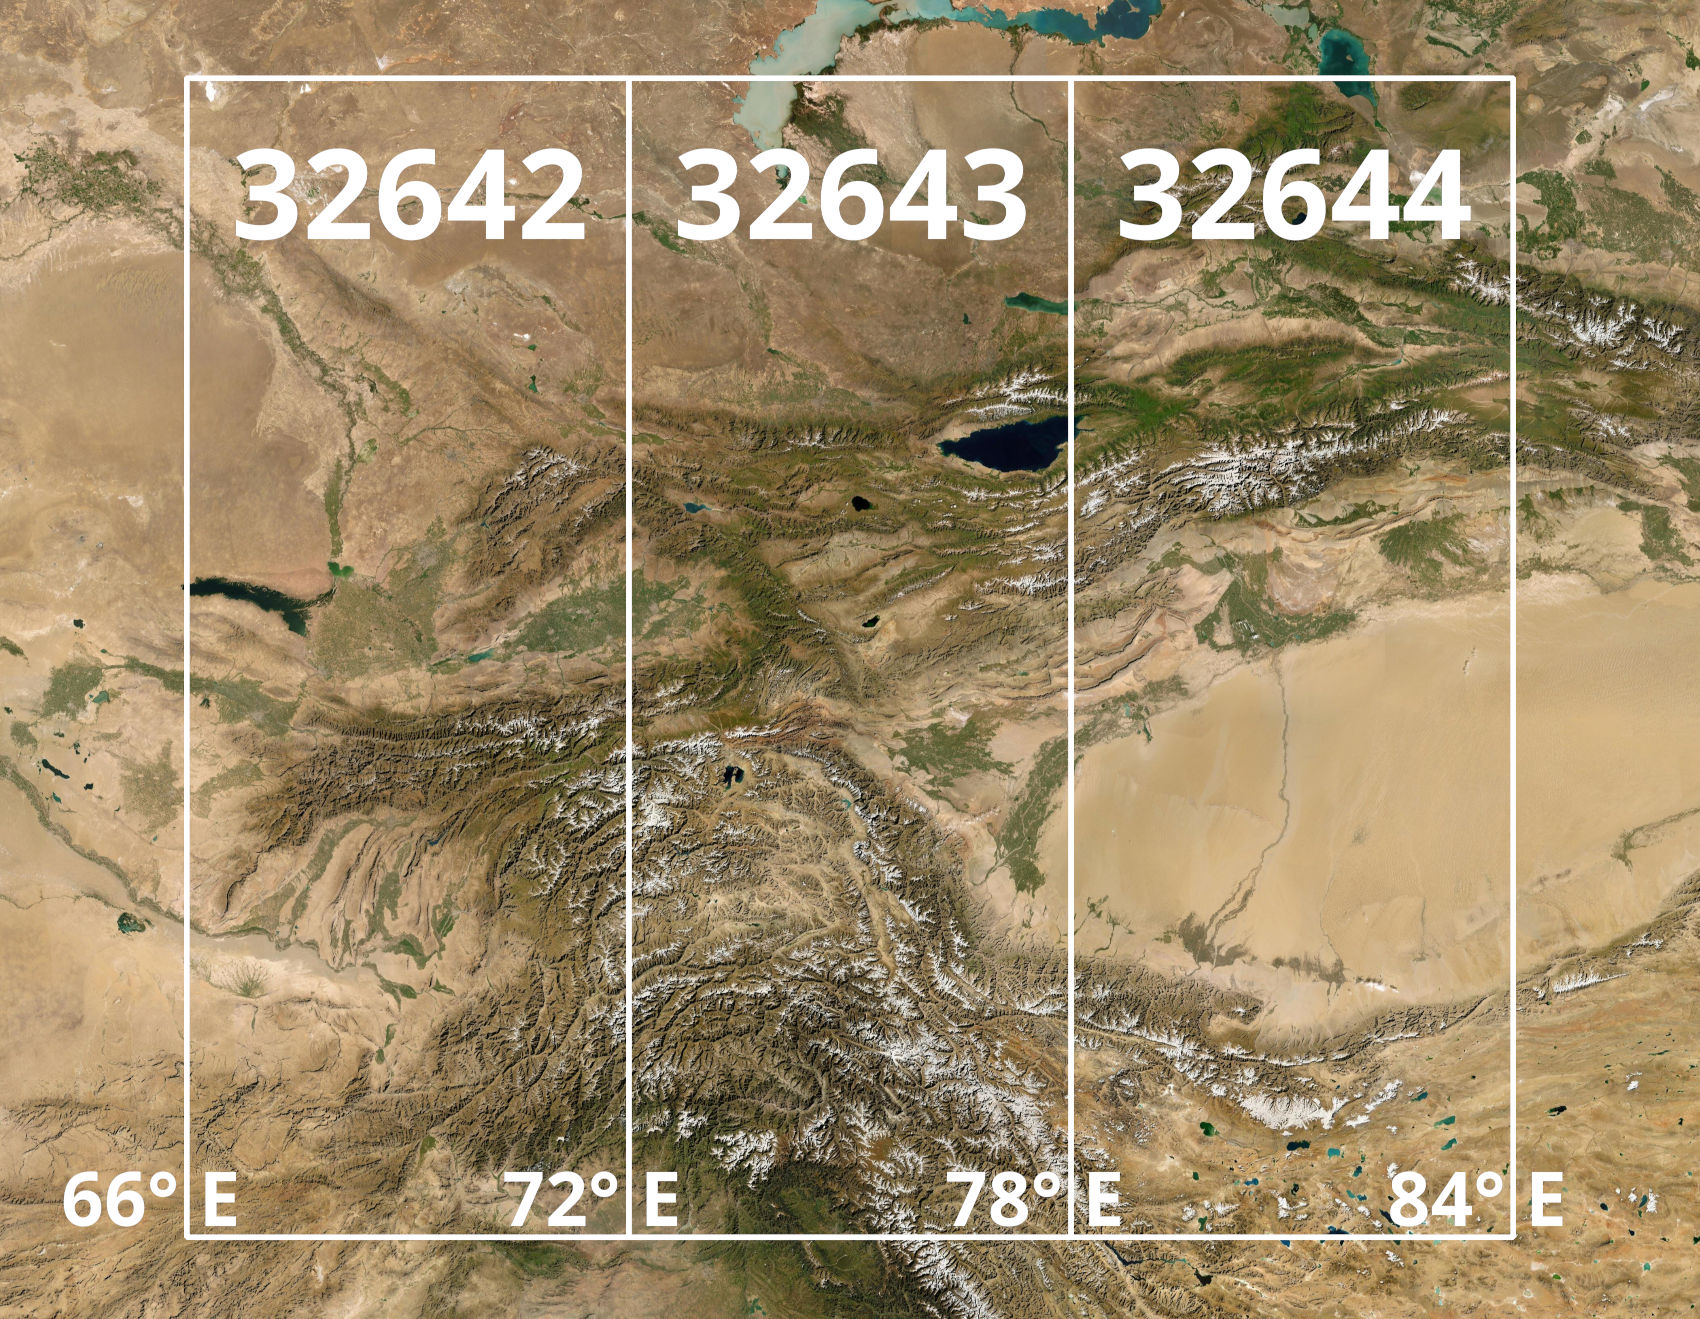
\includegraphics[width=0.56\textwidth]{f10_epsg}
    \caption{The \textbf{EPSG codes} of UTM zones in Central Asia, with their respective longitude borders.}
    \label{fig:f10_epsg}
\end{figure}

\clearpage
\section{Running the model}
After setting the parameters, we can run the model very simply: we just open in RStudio the file \textit{main.R} and we click on \textit{Source} (Fig. \ref{fig:f1_rstudio_source}). While the model is running, we can see the progress in the \textbf{RStudio console} (Fig. \ref{fig:f11_rstudio_console}). In the console the model will show in real time the result of the simulation, as well as \textbf{any error messages.} All messages are also written into a \textbf{log file} (under \textit{logs\textbackslash}).
\vspace{1.0cm}
\begin{figure}[h]
    \centering
    \includegraphics[width=0.85\textwidth]{f11_rstudio_console}
    \caption{The \textbf{RStudio console} with the information messages written by the model.}
    \label{fig:f11_rstudio_console}
\end{figure}


\clearpage
\section{Output files}
The \textbf{model output} is written to a folder called \textit{output\textbackslash yakarcha\textbackslash}. The following \textbf{detailed results} are provided in file \textit{massbalance\_2020.pdf}, under \textit{output\textbackslash yakarcha\textbackslash annual\_results\textbackslash}:

\begin{itemize}
    \item Mass balance map over the hydrological year (from 1 October 2019 to 30 September 2020).
    \item Mass balance map over the measurement period (14 August 2019 to 13 September 2020).
    \item Mass balance map over the annual measurement period, with a \textbf{local correction of the model result} based on the stakes (contour-line method). This is called \textbf{"Measurement period (annual, corrected)"}.
    \item Mass balance map over the winter period (1 October 2019 to 30 April 2020).
    \item Input meteorological series (temperature and precipitation).
    \item Daily time series of the cumulative \textbf{mass balance over the entire glacier}, also with the separate components of melt and accumulation.
    \item Daily melt and rainfall amounts, which can be compared to runoff measurements.
    \item Altitudinal profiles of the mass balance, also compared to the stake measurements
    \item Daily time series of mass balance at the stakes.
\end{itemize}

The \textbf{mass balance maps} are also written to individual GeoTiff files (example: \textit{mb\_annual\_hydro\_2020.tif}), which can be used in QGIS or ArcGIS. The other values - including \textbf{daily and total melt, accumulation, mass balance} and \textbf{rainfall} - are written to plain-text CSV files (example: \textit{mb\_daily\_series\_glacier\_2020.csv}).

The model also makes a \textbf{summary of the results} into two \textbf{overview files}: \textit{output\textbackslash yakarcha\textunderscore overview.pdf} and \textit{output\textbackslash yakarcha\textunderscore overview\_areaplot.pdf}.

\end{document}
